\documentclass{xmgr}
%\documentclass[brudnopis]{xmgr}

%\defaultfontfeatures{Scale=MatchLowercase}
%\setmainfont[Numbers=OldStyle,Ligatures=TeX]{Minion Pro}
%\setsansfont[Numbers=OldStyle,Ligatures=TeX]{Myriad Pro}
% for fontspec version < 2.0
\setmainfont[Numbers=OldStyle,Mapping=tex-text]{Minion Pro}
\setsansfont[Numbers=OldStyle,Mapping=tex-text]{Myriad Pro}
%\setmonofont[Scale=0.75]{Monaco}

% Opcjonalnie identyfikator dokumentu
% drukowany tylko z włączoną opcją 'brudnopis':
\wersja   {wersja wstępna [\ymdtoday]}

\author   {Michał Dettlaff}
\nralbumu {164\,622}
\email    {walenty@szczesny.com.pl}

\title    {Zastosowanie algorytmów genetycznych w projektowaniu optymalnego układu klawiatury}
\date     {2011}
\miejsce  {Gdańsk}

\opiekun  {prof. zw. dr hab. inż. Sławomir Wierzchoń}

% dodatkowe polecenia
%\renewcommand{\filename}[1]{\texttt{#1}}

\begin{document}

\begin{abstract}
  Projektowanie optymalnego, ergonomicznego układu klawiatury można potraktować jako problem optymalizacji kombinatorycznej, do rozwiązania którego można zastosować znane metaheurystyki. W poniższej pracy wykorzystany jest do tego celu algorytm genetyczny, w którym chromosomem jest układ klawiszy zakodowany jako permutacja, a funkcja przystosowania odzwierciedla ilość pracy potrzebną do przepisania tekstu za pomocą danego układu. W wyniku zostają utworzone układy klawiatury przystosowane do pisania w języku polskim oraz angielskim. Następnie są one porównane ze standardowymi układami klawiatury (QWERTY, Dvorak), zaprojektowanymi bez udziału komputera, oraz rozwiązaniami znalezionymi przez inne algorytmy.
\end{abstract}
\keywords{
  algorytmy, genetyczne, klawiatura, Dvorak, QWERTY, optymalizacja
}

% tytuł i spis treści
\maketitle
%
% wstęp
\introduction

Standardowy układ klawiatury (rys. 1), mimo swojej wszechobecności oraz pozostawania w użyciu od ponad 100 lat, jest pod wieloma względami nieoptymalny. Układ ten nazywany jest układem QWERTY (od pierwszych liter w górnym rzędzie w jego amerykańskiej wersji) lub układem Scholesa i został zaprojektowany w latach 70 XIX wieku przez Charles'a Lethama Sholesa. QWERTY zastąpił używany wcześniej układ alfabetyczny i miał na celu zapobieganie zacinaniu się mechanizmu maszyny do pisania, jeżeli użytkownik pisał zbyt szybko~\cite{Norman:1988:DOET}. Z tego względu, litery które często występowały obok siebie w języku angielskim, takie jak \emph{i} oraz \emph{e}, zostały umieszczone po przeciwnych stronach klawiatury. Dzięki temu, belki na których znajdowały się klawisze nie zderzały się ze sobą, co zmniejszało prawdopodobieństwo zacięcia się. Mimo że problem zacinania się maszyny został szybko wyeliminowany i to jeszcze na długo przed nadejściem klawiatury komputerowej, układ klawiatury QWERTY pozostaje w powszechnym użyciu aż do dzisiaj i stanowi de facto standard.

\begin{figure}[!tbh]
\centering
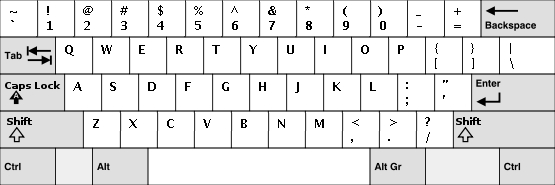
\includegraphics[width=.8\hsize]{fig/qwerty}
\caption{Standardowy układ klawiatury QWERTY}
\source{Opracowanie własne}
\end{figure}

Spośród układów alternatywnych wobec QWERTY największą popularnością cieszy się klawiatura Dvoraka (Dvorak Simplified Keyboard). Została ona zaprojektowana w 1936 r. przez dr Augusta Dvoraka. W przeciwieństwie do QWERTY, podczas jej projektowania nie były już brane pod uwagę ograniczenia mechaniczne maszyn do pisania, ze względu na postępy w ich produkcji. Głównym celem było natomiast umożliwienie efektywnego pisania oraz łatwość nauki. Dvorak sformułował szereg zasad, którymi kierował się podczas projektowania swojego układu klawiszy i które miały pozwolić na osiągnięcie tych celów~\cite{cassingham1986dvorak}. Zgodnie z tymi zasadami, optymalna klawiatura powinna:
\begin{itemize}
\item Uwzględniać statystyczną analizę najczęściej występujących par liter.
\item Zmniejszać prawdopodobieństwo popełniania błędów poprzez uczynienie pisania bardziej "naturalnym" i wygodnym, poprzez zminimalizowanie ruchów palców pomiędzy rzędami klawiszy.
\item Zwiększyć użycie środkowego rzędu (home row) oraz uderzeń pozwalających na jak najszybsze pisanie (takich które wykorzystują pisanie obiema rękami na zmianę, zamiast tą samą ręką przez dłuższy czas).
\item W większym stopniu wykorzystywać prawą rękę, która jest silniejsza w przypadku większości użytkowników.
\item Być łatwiejsza w nauce, przyczyniać się do popełniania mniejszej ilości błędów, oraz minimalizować wysiłek związany z pisaniem.
\end{itemize}
Warto zwrócić uwagę, że cechy statystyczne o których mowa w pierwszym z powyższych punktów są zależne od analizowanego języka. Dvorak przeprowadził analizę dla języka angielskiego, w związku z czym projektowanie klawiatury dla innych języków wiązałoby się z ponownym przeprowadzeniem analizy, a wynikowy układ klawiszy mógłby się znacznie różnić.

Jedną z głównych różnic pomiędzy układem QWERTY a klawiaturą Dvoraka jest przeniesienie najczęściej używanych klawiszy do środkowego rzędu. Dla przykładu, za pomocą samego środkowego rzędu klawiatury Dvoraka można napisać około 400 słów w języku angielskim, natomiast układ QWERTY pozwala w analogiczny sposób napisać tylko około 100 słów~\cite{Call:2005:CME}. Charakterystyczną cechą klawiatury Dvoraka jest umiejscowienie wszystkich samogłosek po tej samej stronie. Wpływa to korzystnie na alternację rąk, ponieważ w języku angielskim samogłoski najczęściej nie występują obok siebie. Klawiatura Dvoraka jest łatwiejsza w nauce i pozwala na około 10\% szybsze pisanie~\cite{Norman:1988:DOET}.

\begin{figure}[!tbh]
\centering
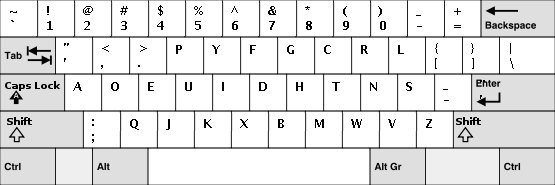
\includegraphics[width=.8\hsize]{fig/dvorak}
\caption{Układ klawiatury Dvorak Simplified Keyboard}
\source{Opracowanie własne}
\end{figure}

Wspomniane układy klawiatury zostały zaprojektowane ręcznie, bez udziału komputera. Podjęto też wiele prób rozwiązania problemu szukania optymalnego klawiatury (Keyboard Arrangement Problem - KAP) z użyciem algorytmów ewolucyjnych oraz innych metaheurystyk. Wagner \cite{Eggers2003672} wygenerował układy klawiatury dla języka angielskiego, niemieckiego oraz francuskiego, stosując algorytm mrówkowy (Ant Colony Optimization) oraz szereg kryteriów ergonomicznych. Yin oraz Su \cite{Yin201143} sformułowali problem ogólnie dla różnych typów klawiatur (General Keyboard Arrangement Problem - GKAP) oraz zastosowali do jego rozwiązania algorytm optymalizacji rojowej (Cyber Swarm Optimization). Deshwal oraz Deb \cite{Hindi} zaproponowali nowy projekt klawiatury dla języka Hindi, stosując algorytm genetyczny z reprezentacją układu klawiszy jako czterowymiarowej tablicy.

Podobne algorytmy stosowano również dla niestandardowych klawiatur, na przykład w telefonach komórkowych, na których pisze się z użyciem jednego lub dwóch palców~\cite{Li2006695}. Niniejsza praca dotyczy KAP rozumianego jako poszukiwanie optymalnego układu klawiszy dla standardowej klawiatury, zoptymalizowanego pod kątem techniki pisania bezwzrokowego (\emph{touchtyping}). Pisanie bezwzrokowe zobrazowane jest na ilustracji poniżej.

\begin{figure}[!tbh]
\centering
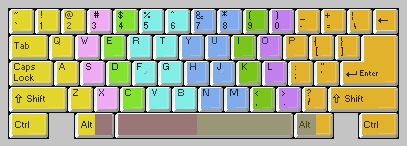
\includegraphics[width=.8\hsize]{fig/touchtyping}
\caption{Użycie palców w pisaniu bezwzrokowym}
\source{Opracowanie własne}
\end{figure}

W technice bezwzrokowej, w domyślnej pozycji palce lewej ręki znajdować się powinny nad klawiszami $asdf$, a prawej nad $jkl;$. Po wciśnięciu któregoś z pozostałych klawiszy, palec powinien powrócić na swoją standardową pozycję w środkowym rzędzie (tzw. home row). Kciuki zajmują się altem i spacją. Kolorami oznaczono, którymi palcami powinno się uderzać poszczególne klawisze, na przykład: lewy serdeczny wciska $x$, $s$, $w$ i $3$, a prawy wskazujący $n$, $m$, $h$, $j$, $y$ itd.

Ocena jakości układu klawiatury opiera się na statystycznych cechach tekstu i ma charakter eksperymentalny. Układy zaprojektowane dotychczas bez udziału komputera były tworzone w dużej mierze w sposób intuicyjny, a stworzenie algorytmu który szukałby optymalnego rozwiązania w sposób analityczny byłoby niezwykle trudne, jeśli nie niemożliwe. W połączeniu z bardzo dużą przestrzenią możliwych rozwiązań (mającą rozmiar $30!$ dla 30 klawiszy), skłania to zastosowania metod metaheurystycznych, do jakich zaliczają się algorytmy genetyczne. Zaletą algorytmów genetycznych jest to, że nie wymagają one do działania żadnych informacji pomocniczych o rozwiązywanym problemie, a tylko funkcję oceny rozwiązania~\cite{Goldberg:1998:AGZ}.

KAP jest przykładem problemu optymalizacji kombinatorycznej. Do klasycznych przykładów zagadnienia optymalizacji kombinatorycznej należy m.in. problem komiwojażera (Travelling Salesman Problem - TSP), który często stosowany jest do porównywania wydajności algorytmów metaheurystycznych. Algorytmy genetyczne były wielokrotniego stosowane z powodzeniem do tego rodzaju problemów, w tym również do TSP~\cite{Michalewicz:2003:AGSDPE}~\cite{Brady}~\cite{Stutzle:2000:CNI:645825.668943}, co pozwala na przypuszczenie że uzyskane wyniki będą zadowalające również dla KAP. Ponadto, istnieje wiele operatorów genetycznych które zaprojektowano z myślą o ścieżkowej reprezentacji TSP~\cite{Larranaga99geneticalgorithms}. Stosując podobną reprezentację problemu w przypadku KAP, możliwe jest ich ponowne wykorzystanie, bez konieczności projektowania genetycznych operatorów od nowa. Należące do nich operatory krzyżowania stworzono głównie z myślą o przekazywaniu informacji o kolejności elementów lub ich pozycjach bezwzględnych między osobnikami. Szczególnie ten drugi rodzaj operatorów jest korzystny dla KAP, ponieważ ocena układu klawiatury zależy głównie od bezwzględnych pozycji poszczególnych klawiszy.

Kolejny rozdział poświęcony jest ogólnemu wprowadzeniu do tematyki algorytmów genetycznych, z opisem schematu algorytmu oraz podstawowych operatorów genetycznych. Następnie, zostanie opisany algorytm genetyczny przystosowany do problemu KAP, z odpowiednio dobraną funkcją przystosowania oraz operatorami mutacji, selekcji i krzyżowania. W kolejnym rozdziale zostaną omówione wyniki działania tego algorytmu dla tekstów w języku polskim oraz angielskim. Uzyskane wyniki porównane są z tymi uzyskanymi przez znane układy klawiatury zaprojektowane ręcznie, oraz układy wygenerowane za pomocą innych algorytmów. Układy wygenerowane przez algorytm uzyskują wyraźną przewagę, zwłaszcza w przypadku wyników dla języka polskiego. W zakończeniu pracy przedstawione zostaną uzyskane konkluzje oraz plany dalszych badań.


\chapter{Algorytmy genetyczne}

Algorytmy genetyczne to rodzaj algorytmów heurystycznych pozwalających na efektywne przeszukiwanie przestrzeni rozwiązań w poszukiwaniu optymalnego rozwiązania. Inspiracją dla algorytmów genetycznych jest ewolucja naturalna, w szczególności mechanizmy dziedziczenia oraz doboru naturalnego. Wykorzystują one biologicznie inspirowane operatory, do których należą rozrodczość, selekcja, mutacja oraz krzyżowanie. Autorem pierwszej publikacji o algorytmach genetycznych która uzyskała szerokie uznanie jest John Holland~\cite{Holland1975}.

Algorytmy genetyczne należą do metod populacyjnych, w których operujemy na pewnym zmieniającym się zbiorze (populacji) rozwiązań. Daje to znaczącą przewagę nad prostszymi algorytmami wspinaczkowymi, w których zachowujemy tylko jedno rozwiązanie w danym momencie. Zachowywanie populacji rozwiązań zmniejsza prawdopodobieństwo przedwczesnej zbieżności w lokalnym optimum, zwiększając możliwości eksploracyjne algorytmu. Inne skrajne podejście, w którym przeszukujemy jednocześnie całą przestrzeń rozwiązań, jest również mało skuteczne ze względu na zbyt duży rozmiar tej przestrzeni dla większości interesujących problemów. Algorytm genetyczny unika tego problemu poprzez dobranie rozmiaru populacji znacznie mniejszego od rozmiaru całej przestrzeni poszukiwań.

Schemat algorytmu genetycznego można przedstawić za pomocą następującego pseudokodu:

\noindent
\rule{360pt}{0.5pt}\newline
\texttt{i := 0\newline
Zainicjuj populację początkową P(i)\newline
Oceń osobniki z populacji początkowej\newline
Powtarzaj dopóki nie jest spełniony warunek zakończenia:\newline
\indent i := i + 1\newline
\indent Wybierz osobniki z P(i-1) i utwórz nową populację P(i)\newline
\indent Zmień osobniki z P(i)\newline
\indent Oceń osobniki z P(i)\newline
}
\rule{360pt}{0.5pt}

Warunkiem zakończenia może być upłynięcie określonej ilości iteracji, lub znalezienie rozwiązania które jest wystarczająco bliskie optimum. Rolę operacji \texttt{Zmień osobniki} w algorytmach genetycznych pełnią mutacja oraz krzyżowanie.

Algorytm genetyczny operuje na osobnikach w zakodowanej postaci, którą najczęściej nazywa się chromosomem. Każdy chromosom reprezentuje potencjalne rozwiązanie zadania. W klasycznych algorytmach genetycznych, chromosom ma postać ciągu bitów o stałej długości.

Pierwszym krokiem algorytmu jest wygenerowanie populacji początkowej. Powinna się ona cechować możliwie dużą różnorodnością, dlatego najczęściej stosowaną metodą jej tworzenia jest generowanie chromosomów w sposób losowy. Czasem w populacji początkowej umieszcza się też specjalnie przygotowane osobniki, o których spodziewamy się że leżą w pobliżu optimum.

Zaletą klasycznych algorytmów genetycznych jest fakt, że uniwersalna reprezentacja chromosomów jako ciągów bitów pozwala na ponowne wykorzystanie tych samych operatorów mutacji oraz krzyżowania. Jedyne co trzeba zrobić aby zastosować algorytm genetyczny do nowego problemu, jest zaimplementowanie funkcji oceny oraz zakodowanie potencjalnych rozwiązań w postaci ciągu bitów. Takie podejście jest jednak problematyczne dla wielu zastosowań. Mutacja oraz krzyżowanie mogą prowadzić do powstawania osobników które stanowią rozwiązanie nieprawidłowe, które muszą zostać odrzucone.

Algorytmy genetyczne znajdują szerokie zastosowania w zadaniach przeszukiwania oraz optymalizacji. Należą do nich między innymi: wytyczanie trasy połączeń kablowych, harmonogramowanie, sterowanie adaptacyjne, rozgrywanie gier, modelowanie poznawcze, zadania transportowe, zadanie komiwojażera, sterowanie optymalne oraz optymalizacja obsługi zapytań w bazach danych~\cite{Michalewicz:2003:AGSDPE}.

\section{Selekcja}

Wybór osobników do nowo tworzonych populacji jest procesem analogicznym do doboru naturalnego. W ujęciu Karola Darwina, największe szanse przetrwania mają osobniki najlepiej przystosowane do środowiska. Wpływ środowiska jest w algorytmach genetycznych modelowany przez funkcję oceny lub funkcję przystosowania. Ponieważ problemy optymalizacji zwykle definiuje się w kategoriach poszukiwania minimum, przyjmiemy konwencję zgodnie z którą mniejsza wartość funkcji oceny oznacza lepsze przystosowanie. Dlatego też w operacji wyboru (selekcji) osobników do nowej populacji powinny być faworyzowane osobniki o niższej wartości funkcji przystosowania.

Jedną z najprostszych implementacji operacji selekcji jest selekcja proporcjonalna, w której osobniki wybierane są z prawdopodobieństwem proporcjonalnym do wartości funkcji przystosowania. Wadą selekcji proporcjonalnej jest tendencja do zbyt szybkiego zdominowania populacji przez najbardziej przystosowane osobniki. Dlatego zaproponowano wiele alternatywnych implementacji operatora selekcji, takie jak selekcja rangowa, turniejowa, lub podwójna turniejowa.

Selekcja turniejowa to bardzo prosty algorytm selekcji, będący jednocześnie jednym z najpopularniejszych~\cite{Luke2009Metaheuristics}. W selekcji turniejowej, wybieramy najlepiej przystosowanego osobnika spośród losowo wybranego podzbioru populacji, bez powtórzeń. Algorytm można dostosować poprzez zmianę parametru $t$, czyli rozmiaru wybieranego podzbioru. Innymi zaletami algorytmu są jego prostota oraz niezależność od szczegółów implementacji funkcji przynależności.

Pseudokod:

\noindent
\rule{380pt}{0.5pt}\newline
\texttt{WEJŚCIE: populacja, t - rozmiar turnieju\newline
Best := wybierz bez zwracania osobnika z populacji\newline
Powtarzaj t - 1 razy:\newline
\indent Next := wybierz bez zwracania osobnika z populacji\newline
\indent jeżeli Next ma korzystniejszą wartość przystosowania niż Best:\newline
\indent\indent Best := Next\newline
zwróć Best\newline
}
\rule{380pt}{0.5pt}\newline

Najczęściej wybieraną wartością parametru $t$ w przypadku algorytmów genetycznych jest 2~\cite{Luke2009Metaheuristics}.

Sam operator selekcji nie jest wystarczającym warunkiem do tego, aby wartość funkcji oceny poprawiała się w kolejnych populacjach. Potrzebny jest operator wprowadzający zmienność oraz innowacje do populacji. W klasycznych algorytmach genetycznych, służą do tego operacje mutacji oraz krzyżowania.

\section{Mutacja}

Operacja mutacji powinna powodować jedynie niewielką zmianę w położeniu rozwiązania w pejzażu dostosowań. To znaczy, niewielka modyfikacja chromosomu powinna wpływać w niewielkim stopniu na wartość funkcji przystosowania. W klasycznym algorytmie genetycznym, mutacja polega na losowej zmianie elementu chromosomu z jednakowym (niewielkim) prawdopodobieństwem na wartość przeciwną (z jedynki na zero i na odwrót) \cite{Goldberg:1998:AGZ}.

\section{Krzyżowanie}

Jednym z prostszych operatorów krzyżowania dla binarnej reprezentacji chromosomu jest krzyżowanie punktowe. W krzyżowaniu punktowym, wybieramy na chromosomie losowo punkt przecięcia. Aby utworzyć pierwszego potomka, kopiujemy geny leżące na lewo od punktu przecięcia z jednego rodzica, a geny leżące na prawo z drugiego rodzica. Drugi potomek powstaje analogicznie poprzez skopiowanie najpierw prawej, a następnie lewej strony. Przykładowo, w wyniku zastosowania krzyżowania punktowego z punktem przecięcia między drugą i trzecią pozycją do pary rodziców:
$$(a_1 a_2 a_3 a_4 a_5), (b_1 b_2 b_3 b_4 b_5)$$

otrzymamy następujące osobniki potomne:
$$(a_1 a_2 b_3 b_4 b_5), (b_1 b_2 a_3 a_4 a_5)$$

Wadą krzyżowania punktowego jest fakt, że geny leżące na sąsiadujących pozycjach będą rozdzielane z większym prawdopodobieństwem od genów leżących na bardziej odległych pozycjach. Jednym ze sposobów na zniwelowanie tego problemu jest zwiększenie liczby punktów przecięcia, w wyniku czego otrzymamy krzyżowanie wielopunktowe.


\chapter{Opis algorytmu}


\section{Reprezentacja chromosomu}

Układ klawiatury można zakodować jako ciąg binarny, opisując każdy klawisz za pomocą określonej ilości bitów. Niestety, stosowanie klasycznych operatorów genetycznych spowoduje, że zdecydowana większość powstałych w ten sposób rozwiązań będzie nieprawidłowych. Przykładowo, jeżeli użyjemy trzech bitów do opisania każdego klawisza klawiatury o 40 klawiszach, tylko jedna z każdych 1016 dowolnie wybranych struktur 120-bitowych jest strukturą o właściwej konfiguracji klawiszy~\cite{GloverKey}.

W związku z powyższym, zastosowana zostanie permutacyjna reprezentacja chromosomu oraz specjalnie dla niej dostosowane operatory mutacji oraz krzyżowania. Układ klawiatury reprezentowany jest przez permutację 30 klawiszy. 26 klawiszy oznaczanych jest literami alfabetu łacińskiego A-Z, a pozostałe odpowiadają znakom ",", ".", "?" oraz ";". Wynika z tego, że liczba wszystkich możliwych układów klawiatury wynosi $$ 30! \simeq 2.65 * 10^{32} $$ co stanowi rozmiar przestrzeni poszukiwań na której będzie działał algorytm genetyczny. Zbiór wszystkich znaków wchodzących w skład permutacji oznaczymy jako $ A $.

Klawisze podzielone są na trzy grupy, gdzie pierwsze 10 oznacza klawisze górnego rzędu klawiatury, następne 10 klawisze rzędu środkowego, a ostatnie 10 - dolnego rzędu.

Dla przykładu, układ klawiatury QWERTY jest reprezentowany przez następującą permutację:
$$ (qwertyuiopasdfghjkl;zxcvbnm,.?) $$


\section{Funkcja przystosowania}

Naszym celem jest znalezienie układu klawiatury, który przyczyni się do zwiększenia prędkości pisania oraz zminimalizowania zmęczenia palców użytkownika. Inne pożądane cechy to minimalizowanie ilości błędów oraz łatwość nauki danego układu klawiatury. Dlatego też te cele będą brane pod uwagę podczas projektowania funkcji przystosowania algorytmu genetycznego.

W kolejnych podrozdziałach zostaną opisane kryteria, które składają się na funkcję przystosowania. Zostały opracowane głównie w oparciu o prace Wagnera~\cite{Eggers2003672} oraz Dvoraka~\cite{cassingham1986dvorak}. Ostateczna postać funkcji przystosowania jest sumą ważoną wyników z poszczególnych kryteriów.

Do obliczania oceny układu klawiatury wykorzystywane są zbiory tekstów, stanowiących możliwie reprezentatywną próbkę z danego języka. Wynikowy układ powinien być jak najlepiej przystosowany do przepisywania podanego tekstu, dlatego użyte zostaną osobne zbiory tekstów dla języka polskiego oraz angielskiego. Naiwnym sposobem na obliczenie przystosowania byłaby symulacja przepisywania tekstu, wymagająca analizy całości tekstu za każdym razem od nowa podczas obliczania funkcji przystosowania. Takie podejście jest jednak zbyt kosztowne obliczeniowo, ponieważ złożoność funkcji przystosowania wyniosłaby $ O(n) $, gdzie $ n $ stanowiące długość tekstu byłoby wartością rzędu $ 10^5 $ lub $ 10^6 $.

Z tego powodu funkcja przystosowania nie będzie obliczana na podstawie oryginalnego tekstu, ale jego cech statystycznych, które będą obliczane tylko raz przed uruchomieniem algorytmu. W ten sposób czas obliczania funkcji przystosowania nie będzie zależny od długości tekstu (jego złożoność wyniesie $ O(1) $). Cechy statystyczne tekstu zostaną opisane za pomocą dwóch funkcji:
$$ f_m : M \rightarrow \mathrm{R} $$
$$ f_d : D \rightarrow \mathrm{R} $$

Do opisania tych funkcji przydatne będą dwie definicje. Jako \emph{monograf} będziemy rozumieć rodzaj zdarzenia polegającego na naciśnięciu klawisza któremu odpowiada element chromosomu. Wpływ pozostałych klawiszy zostanie pominięty~-~przykładowo, zakładamy że podczas wpisywania wielkich liter klawisz SHIFT zostaje uderzony przeciwną ręką do tej, która uderza klawisz z literą. \emph{Diagraf} natomiast definiujemy jako parę monografów następujących zaraz po sobie. Przykładowo, w tekście o treści \emph{barbaz} możemy wyróżnić 4 monografy: \emph{b}, \emph{a}, \emph{r} oraz \emph{z}, oraz 4 diagrafy: \emph{ba}, \emph{ar}, \emph{rb}, oraz \emph{az}. Dziedzinę funkcji $ f_m $ będziemy określać jako zbiór wszystkich monografów $ M $, a dziedzinę funkcji $ f_d $ jako zbiór wszystkich możliwych diagrafów $ D $.
$$ M = \{ a : a \in A \} $$
$$ D = \{ ab : a \in A, b \in A \} $$

$ f_m $ opisuje częstotliwości występowania monografów w zbiorze tekstów, a $ f_d $ częstotliwości występowania diagrafów. Przez częstotliwość występowania rozumiemy procentowy udział ilości wystąpień danego monografu (diagrafu) w sumie ilości wystąpień wszystkich monografów (diagrafów). Przykładowo, dla tekstu \emph{barbaz} $ f_m(z) = \frac{1}{6} $, a $ f_d(ba) = \frac{2}{5} $.


\subsection{Użycie palców}

Pierwszym czynnikiem branym pod uwagę będzie rozkład pracy na poszczególne palce. Chcemy, aby najczęściej używane były najsilniejsze i najdłuższe palce, a najmniej używane palce najsłabsze.

W tym celu zdefiniujemy optymalny rozkład użycia, który podajemy w oparciu o~\cite{Eggers2003672}. $f^{opt}_1$ do $f^{opt}_4$ oznaczają udział palców lewej ręki w przepisywaniu tekstu, od małego palca do wskazującego, natomiast $f^{opt}_5$ do $f^{opt}_8$ analogicznie udział palców prawej ręki, od wskazującego do małego.\newline

\begin{tabular}{ c | c | c | c | c | c | c | c }
  $f^{opt}_1$ & $f^{opt}_2$ & $f^{opt}_3$ & $f^{opt}_4$ & $f^{opt}_5$ & $f^{opt}_6$ & $f^{opt}_7$ & $f^{opt}_8$ \\
  \hline
  4.4\% & 12.3\% & 15.8\% & 17.5\% & 17.5\% & 15.8\% & 12.3\% & 4.4\% \\
\end{tabular}\newline

Czynnik funkcji przystosowania odpowiadający użyciu palców przyjmie następującą postać, odzwierciedlającą rozbieżność pomiędzy rozkładem otrzymanym a optymalnym:
$$ p_{finger} = \sum\limits_{i = 1}^{8} (f_i^{opt} - f_i)^2 $$


\subsection{Użycie rzędów klawiszy}

Podczas pisania techniką bezwzrokową, pozycją domyślną jest utrzymywanie palców nad klawiszami w środkowym rzędzie (tzw. \emph{home row}). Z tego powodu optymalny układ klawiatury powinien zawierać najczęściej używane znaki w środkowym rzędzie. Znaki z górnego oraz dolnego rzędu wymagają ruchu palca z domyślnego rzędu środkowego, a następnie powrotu na pozycję domyślną, co jest mniej optymalne. Klawisze z górnego rzędu są przy tym nieco łatwiej dostępne od tych z dolnego.

Górny, środkowy oraz dolny rząd klawiszy oznaczymy odpowiednio jako: $R_1$, $R_2$, $R_3$. Jako optymalny rozkład częstotliwości użycia poszczególnych rzędów przyjmiemy rozkład układu klawiatury, w którym 10 najczęściej używanych klawiszy należy do $R_1$, 10 kolejnych do $R_2$, a 10 najmniej używanych klawiszy do $R_3$. Częstotliwości użycia obliczane są na podstawie stosowanego zbioru tekstów.

Przykładowe wartości: $f_{R_1} = 50\%$, $f_{R_2} = 35\%$, $f_{R_3} = 15\%$

Biorąc powyższe kryteria pod uwagę, czynnik funkcji przystosowania dotyczący położenia znaku w danym rzędzie przyjmie następującą postać:
$$ p_{row} = \sum\limits_{i = 1}^{3} (f_{R_i}^{opt} - f_{R_i})^2 $$


\subsection{Alternacja rąk}

Czynnikiem sprzyjającym szybkiemu i komfortowemu pisaniu jest unikanie pisania kolejnych znaków tą samą ręką. Jest to jedna z głównych zasad która została zastosowana przy projektowaniu klawiatury Dvoraka, gdzie w tym celu wszystkie samogłoski umieszczono z lewej strony klawiatury.

Liczbową reprezentacją tej zasady będzie następujące wyrażenie:

$$ p_{hand\_alter} = \sum\limits_{f \in f_{sh}} f $$

Gdzie $ f_{sh} \in f_d $ oznacza zbiór częstotliwości występowania diagrafów pisanych tą samą ręką.


\subsection{Alternacja palców}

Podobnie jak w poprzednim punkcie, nie jest korzystne pisanie kolejnych znaków tym samym palcem. Dodatkowe utrudnienie stanowi sytuacja, w której ten sam palec musi przebyć większą odległość. Dlatego też częstotliwość występowania diagrafów zostanie dodatkowo pomnożona przez współczynnik odległości $dist$.
$$ p_{finger\_alter} = \sum\limits_{d \in D'} f_d dist(d) $$

\noindent
gdzie zbiór $ D' \in D $ oznacza zbiór diagrafów które pisane są tym samym palcem, a $f_d$ oznacza częstotliwości występowania tych diagrafów.\newline

Jako odległość $dist$ zostanie przyjęta odległość Manhattan:
$$ dist(d) = |c_2 - c_1| + |r_2 - r_1| $$

gdzie $c_1$ oraz $r_1$ stanowią współrzędne odpowiednio rzędu i kolumny pierwszego znaku z diagrafu $d$, a $c_2$ oraz $r_2$ współrzędne drugiego znaku diagrafu $d$.


\subsection{Duże ruchy palcami tej samej ręki}

W wypadku użycia tej samej ręki do naciśnięcia kolejno dwóch klawiszy, należy unikać sytuacji w której klawisze te znajdują się daleko od siebie. Dlatego też podczas obliczania tego współczynnika będą brane pod uwagę diagrafy wpisywane tą samą ręką, ale przy użyciu różnych palców, gdzie pionowa odległość jest większa niż jeden rząd (zbiór ten oznaczymy jako $ D' \in D $). W zależność od tego które palce zostaną użyte, zostaną przypisane odpowiednie wagi zgodnie z poniższą tabelą~\cite{Eggers2003672}.\newline

\begin{tabular}{ c | c | c | c | c }
  & wskazujący & środkowy & serdeczny & mały \\
  \hline
  wskazujący & 0 & 5 & 8 & 6 \\
  środkowy & 5 & 0 & 9 & 7 \\
  serdeczny & 8 & 9 & 0 & 10 \\
  mały & 6 & 7 & 10 & 0 \\
\end{tabular}\newline\newline

Wzór przyjmie postać:
$$ p_{step} = \sum\limits_{d \in D'} K(d) f_d $$

gdzie $K(d)$ oznacza współczynnik wagowy przypisany zgodnie z tabelą.


\subsection{Inboard stroke flow}

Dla diagrafów wpisywanych z użyciem tej samej ręki, bardziej korzystny jest kierunek prowadzący do środka, czyli w kierunku od małego palca do wskazującego (tzw. \emph{inboard stroke flow}). Czynnikowi temu będzie odpowiadał następujący wzór, w którym sumujemy częstotliwości występowania diagrafów prowadzących mniej korzystnym kierunku (zbiór takich diagrafów oznaczymy poniżej jako $ D' \in D $):

$$ p_{isf} = \sum\limits_{d \in D'} f_d $$


\subsection{Użycie rąk}

Wysiłek związany z pisaniem powinien być rozłożony proporcjonalnie na obie ręce. Dvorak~\cite{cassingham1986dvorak} oraz część innych autorów~\cite{Call:2005:CME} sugeruje, aby faworyzować w niewielkim stopniu prawą, silniejszą rękę. Przyjmiemy tutaj, że w idealnym przypadku prawa ręka powinna wykonywać 52,5\% pracy związanej z pisaniem. Czynnik ten wyniesie zatem:
$$ p_{hand\_usage} = (f_{left} - 47,5\%)^2 + (f_{right} - 52,5\%)^2 $$

gdzie $f_{left}$ oznacza procentowy udział znaków wpisanych lewą ręką, a $f_{right}$ analogicznie prawą ręką.\newline\newline


\noindent Ostatecznie, funkcja przystosowania przyjmie postać:
$$ p = p_{finger} w_{finger} + p_{row} w_{row} + p_{hand\_alter} w_{hand\_alter} + p_{finger\_alter} w_{finger\_alter} + $$
$$ p_{step} w_{step} + p_{isf} w_{isf} + p_{hand\_usage} w_{hand\_usage} $$

\noindent
gdzie \emph{w} są wagami poszczególnych składowych. Wagi dobrane są eksperymentalnie w ten sposób, aby poszczególne czynniki miały zbliżony wpływ na ostateczną wartość funkcji przystosowania.


\section{Operatory krzyżowania}

\subsection{Krzyżowanie cykliczne (CX)}

Istotną cechą jaką powinien posiadać algorytm krzyżowania do naszych zastosowań, jest zachowywanie absolutnych pozycji elementów w chromosomie. Cechę tę posiada operator krzyżowania cyklicznego~\cite{Oliver}. Średnio połowa absolutnych pozycji elementów z obu rodziców zostaje w nim zachowana.

W krzyżowaniu cyklicznym, wybieramy losowy element z losowo wybranego rodzica i umieszczamy go na tej samej pozycji w chromosomie potomnym. Procedura ta musi być odpowiednio zmodyfikowana, aby zapewnić że chromosom potomny stanowi prawidłową permutację (a zatem prawidłowy układ klawiatury).

Jeżeli okazuje się, że danego elementu z chromosomu rodzica nie można umieścić w chromosomie potomnym, zostaje wybrany element drugiego rodzica. Jeżeli ten element również nie może zostać wybrany, zostaje wybrany losowo jeden z pozostałych elementów, które są dozwolone. Kolejne elementy wybrane z jednego rodzica tworzą jeden cykl, stąd nazwa algorytmu.

Rozważmy przykład. Niech dane będą następujące osobniki rodzicielskie:
$$ (a b c d e f g h), (b d f h g e c a) $$

Na początku musimy wybrać pozycję, z której będzie pochodził pierwszy element. Załóżmy, że będzie to pierwsza. Na pierwszą pozycję chromosomu potomka możemy teraz wybrać $a$ lub $b$, w zależności od tego który rodzic zostanie wybrany. Niech będzie to rodzic pierwszy. Chromosom osobnika potomnego wyglądać będzie następująco (gwiazdką zaznaczono pozycje jeszcze nieprzypisane):
$$ (a * * * * * * *) $$

Rozpatrzmy teraz element na ostatniej pozycji. Możemy wybrać $a$ lub $h$, ale jeżeli wybierzemy $a$, wynikowy chromosom nie będzie już prawidłową permutacją. Dlatego wybieramy $h$.
$$ (a * * * * * * h) $$

Geny na czwartej oraz drugiej pozycji muszą również zostać wybrane z pierwszego rodzica, aby uniknąć wybrania po raz kolejny tych samych elementów.
$$ (a b * d * * * h) $$

Ponieważ wszystkie do tej pory wybrane elementy należą do tego samego rodzica, możemy powiedzieć że tworzą one cykl. Rozpatrzmy teraz elementy na trzeciej pozycji. Możemy wybrać dowolny z nich ($c$ lub $f$). Jeżeli wybierzemy element z drugiego rodzica ($f$), wtedy elementy na piątej, szóstej i siódmej pozycji również mogą pochodzić z drugiego rodzica, tworząc drugi cykl. Ostatecznie, otrzymujemy następującego osobnika potomnego:
$$ (a b f d g e c h) $$


\subsection{Krzyżowanie z częściowym odwzorowaniem (PMX)}

Podobnie jak krzyżowanie cykliczne, krzyżowanie z częściowym odwzorowaniem~\cite{GoldbergLingle} zachowuje częściowo absolutne pozycje elementów rodzicielskich. Fragment chromosomu jednego z rodziców jest przepisywany na potomka, a pozostała część chromosomu jest tworzona na podstawie odwzorowań.

Na początku, wybierane są losowo dwa punkty w chromosomie. Fragment znajdujący się pomiędzy nimi nazywać będziemy \emph{sekcją odwzorowania}. Sekcja odwzorowania drugiego rodzica przepisywana jest na te same pozycje do pierwszego potomka, a sekcja odwzorowania pierwszego rodzica - do drugiego potomka. Następnie, pozostałe pozycje potomka przepisywane są z odpowiadającego mu rodzica, chyba że przepisywany element już istnieje w chromosomie potomka - w takim wypadku brany jest inny element, na podstawie odwzorowania określonego przez sekcje odwzorowania.

Dla przykładu, niech dane będą następujące osobniki rodzicielskie:
$$ (a b c d e f g h), (c g e a f h b d) $$

Załóżmy, że wylosowano punkty pomiędzy trzecim i czwartym, oraz szóstym i siódmym elementem chromosomu, co daje sekcję odwzorowania od czwartego do szóstego elementu. Po przepisaniu sekcji odwzorowania, osobniki potomne mają następującą postać:
$$ (* * * a f h * *), (* * * d e f * *) $$

Sekcje odwzorowania $ (a f h) $ oraz $ (d e f) $ definiują odwzorowania: $ a \leftrightarrow d $, $ f \leftrightarrow e $ oraz $ h \leftrightarrow f $. Przypiszmy teraz brakujące elementy pierwszego potomka. Pierwszym elementem pierwszego rodzica jest $a$. Nie możemy jednak przepisać go na pierwszą pozycję potomka, ponieważ element ten występuje już w permutacji. Możemy jednak przypisać $d$, ponieważ zgodnie z odwzorowaniami $a$ jest odwzorowany na $d$.
$$ (d * * a f h * *) $$

Elementy na drugiej, trzeciej oraz siódmej pozycji można przepisać bezpośrednio, ponieważ nie powodują one powstawania nieprawidłowej permutacji.
$$ (d b c a f h g *) $$

Aby uzupełnić ostatnią pozycję, trzeba zastosować odwzorowanie dwukrotnie. Nie możemy przepisać $h$, więc najpierw stosujemy odwzorowanie $h \rightarrow f$. $f$ także występuje już w permutacji, dlatego odwzorowujemy $f \rightarrow e$.
$$ (d b c a f h g e) $$

Warto zwrócić uwagę, że pozycje sześciu z ośmiu elementów zostały zachowane. Drugi potomek powstaje analogicznie, przez stosowanie tych samych reguł.


\subsection{Krzyżowanie bazujące na porządku (POS)}

Operator POS~\cite{Syswerda} również należy do kategorii operatorów, które mają na celu zachowanie tych samych pozycji dla jak największej ilości elementów chromosomów rodzicielskich. Na początku wybierany jest losowo zbiór pozycji na chromosomie. Elementy na tych pozycjach są przepisywane na te same pozycje z drugiego rodzica do pierwszego potomka i odwrotnie. Niech dane będą pozycje trzecia, czwarta i piąta, oraz osobniki rodzicielskie:
$$ (a b c d e f), (e d b f a c) $$

Po przepisaniu elementów na danych pozycjach, otrzymujemy osobniki potomne:
$$ (* * b f * c), (* * c d * f) $$

Pozostałe pozycje pierwszego potomka wypełniane są kolejnymi elementami pierwszego rodzica, przy czym elementy powtarzające się są pomijane. Element $a$ zostaje przepisany na tą samą, pierwszą pozycję, $b$ i $c$ są pomijane, $d$ zostaje przepisany na kolejną wolną pozycję (drugą), a $e$ na pozycję piątą. Stosując analogiczną procedurę dla drugiego potomka, otrzymujemy w wyniku:
$$ (a d b f e c), (e b c d a f) $$


\subsection{Krzyżowanie naprzemienne (AP)}

Ten typ krzyżowania polega na wybieraniu elementów na przemian z pierwszego i drugiego rodzica~\cite{Larranaga99geneticalgorithms}. Jeżeli dany element znajduje się już w chromosomie osobnika potomnego, jest on zwyczajnie pomijany. Przykładowo, niech będą dane osobniki rodzicielskie $(a b c d e f g h)$ oraz $(d c h b e f g a)$. Zaczynając od pierwszej pozycji, dobieramy najpierw element z pierwszej pozycji pierwszego rodzica, a następnie z pierwszej pozycji drugiego rodzica. Czynność tę powtarzamy dla drugiej pozycji, otrzymując:
$$ (a d b c * * * *) $$

Następny w kolejności element $c$ z pierwszego rodzica występuje już w osobniku potomnym, dlatego pomijamy go i wstawiamy następny element, jakim jest $h$ z drugiego rodzica. Ostatecznie, otrzymamy następującego osobnika potomnego:
$$ (a d b c h e f g) $$

Drugi osobnik potomny powstaje przez przeprowadzenie analogicznej procedury z odwróconą kolejnością osobników rodzicielskich:
$$ (d a c b h e f g) $$


\section{Operatory mutacji}

\subsection{Operator zamiany (EM)}

Operator zamiany~\cite{Larranaga99geneticalgorithms} polega na wybraniu losowo dwóch elementów permutacji, a następnie zamienieniu ich miejscami. Na przykład, jeżeli w permutacji $ (a b c d e f g h) $ wybierzemy element drugi i piąty, otrzymamy w efekcie:
$$ (a \textit{\textbf{e}} c d \textit{\textbf{b}} f g h) $$

\subsection{Zamiana z przemieszczeniem (DM)}

Pierwszym krokiem w metodzie zamiany z przemieszczeniem~\cite{Michalewicz:2003:AGSDPE} jest wybranie losowego odcinka permutacji. Załóżmy, że zaczęliśmy od permutacji $ (a b c d e f g h) $ i wybraliśmy odcinek $ (d e f g) $. Następnie, należy usunąć wybrany odcinek z permutacji i umieścić go w niej ponownie na losowo wybranej pozycji. W naszym przykładzie, po jego usunięciu permutacja przyjmie postać:
$$ (a b c h) $$

Załóżmy, że w tak powstałej permutacji wylosowano pozycję pomiędzy elementami $a$ oraz $b$. W takim wypadku, ostateczny wynik mutacji przyjmie następującą postać:
$$ (a \textit{\textbf{defg}} b c h) $$

\subsection{Prosta inwersja (SIM)}

Operator prostej inwersji~\cite{Holland1975} polega na odwróceniu kolejności elementów w wybranym fragmencie chromosomu. Przykładowo, niech dany będzie chromosom:
$$ (a b c d e f g h) $$

Najpierw należy wybrać dwa punkty cięcia - niech będą to punkty pomiędzy elementami $a$ i $b$, oraz $e$ i $f$. Następnie fragment chromosomu pomiędzy punktami cięcia zostaje odwrócony, dając w efekcie następujący wynik:
$$ (a \textit{\textbf{edcb}} f g h) $$

\subsection{Mutacja z mieszaniem podlist (SM)}

Podobnie jak w poprzednim przypadku, ten rodzaj mutacji również rozpoczyna od wyboru dwóch punktów cięcia definiujących fragment chromosomu~\cite{Syswerda}. Następnie, dokonywana jest losowa permutacja elementów na wybranym fragmencie. Załóżmy, że wybrany został fragment $(b c d)$ z poniższego chromosomu:
$$ (a b c d) $$

W takim wypadku istnieje sześć możliwych rezultatów, do których należą:
$$(\textit{\textbf{abc}} d), (\textit{\textbf{acb}} d), (\textit{\textbf{bac}} d), (\textit{\textbf{bca}} d), (\textit{\textbf{cab}} d), (\textit{\textbf{cba}} d) $$

\subsection{Inwersja (IVM)}

Operator IVM~\cite{Fogel1993} działa podobnie jak DM, z tą różnicą, że dodatkowo odwracana jest kolejność elementów w wybranym fragmencie chromosomu. Niech dany będzie chromosom $ (a b c d e f g h) $. Załóżmy, że podobnie jak w przypadku operatora DM wybraliśmy odcinek $ (d e f g) $, a na jego nową pozycję wybrany został punkt pomiędzy elementami $a$ oraz $b$. Przed ponownym umieszczeniem odcinka w chromosomie, najpierw zostanie odwrócona kolejność jego elementów:
$$ (d e f g) \rightarrow (g f e d) $$
Spowoduje to powstanie następującego wyniku końcowego:
$$ (a b c \textit{\textbf{gfed}} h) $$

\subsection{Mutacja ze wstawianiem (ISM)}

Ten rodzaj mutacji~\cite{Michalewicz:2003:AGSDPE} polega na wybraniu losowego elementu chromosomu, usunięciu go, a następnie wstawieniu ponownie na innej pozycji. Na przykład, po wybraniu elementu szóstego z chromosomu $(a b c d e f g h)$, usunięciu go, a następnie wstawieniu ponownie na pozycji drugiej otrzymamy następujący wynik:
$$ (a \textit{\textbf{f}} b c d e g h) $$

Warto zwrócić uwagę, że jeśli wybrane punkty będą znajdowały się na odległych pozycjach, zmienią się absolutne pozycje wszystkich elementów znajdujących się pomiędzy nimi. Może mieć to bardzo negatywny wpływ na jakość rozwiązania, zwłaszcza ze względu na czynnik stopnia użycia poszczególnych palców.


\section{Optymalizacja dla wielu kryteriów}

W funkcji oceny uwzględnianych jest 7 różnych kryteriów, co sprawia że rozwiązywany problem należy do klasy problemów optymalizacji wielokryterialnej. Najbardziej pożądaną sytuacją jest znalezienie rozwiązania nie tylko z najkorzystniejszą wartością funkcji przystosowania, ale też takiego, które będzie optymalne pod względem każdego ze stosowanych kryteriów. Trudno jest osiągnąć ten cel poprzez samo dobieranie wag ($w_1 ... w_7$), ponieważ często poszczególnych kryteriów nie daje się w łatwych sposób porównać. Dlatego zastosowany zostanie operator selekcji uwzględniający nie tylko wartość funkcji przystosowania, ale również wartości poszczególnych kryteriów.

W optymalizacji wielokryterialnej często stosuje się pojęcie \emph{dominacji Pareto}. Jeżeli za funkcję celu $f$ przyjmiemy wartość przyjmowaną przez dane kryterium (lub cel), mówimy że rozwiązanie A dominuje w sensie Pareto nad rozwiązaniem B jeżeli $f(A)$ jest co najmniej tak dobre jak $f(B)$ dla wszystkich celów, i lepsze dla co najmniej jednego celu ($k$ to ilość celów):
$$ \left( \forall i \right) \left( f_i(A) \le f_i(B) \right) \wedge \left( \exists i \right) \left( f_i(A) \textless f_i(B) \right), \hspace{8pt} 1 \le i \le k $$

Przez rozwiązanie \emph{zdominowane} rozumiemy takie, dla którego istnieje inne rozwiązanie które dominuje nad nim. Rozwiązanie \emph{niezdominowane} to takie, dla którego nie istnieje inne rozwiązanie nad nim dominujące.

Istnieją algorytmy genetyczne wykorzystujące pojęcie dominacji Pareto. Jednym z nich jest NSGA~\cite{SrinivasDeb} (Non-Dominated Sorting Genetic Algorithm), który porównuje osobniki ze względu na ich \emph{rangę Pareto}. Osobniki niezdominowane w danej populacji mają rangę równą 1. Po ich usunięciu z populacji, nowy zbiór osobników niezdominowanych ma przypisaną rangę 2, i tak dalej. Istnieje też kolejna wersja tego algorytmu nazwana NSGA-II, różniąca się zastosowaniem elitarności. Innym przykładem algorytmu genetycznego do optymalizacji wielokryterialnej jest VEGA~\cite{Shaffer1984} (Vector Evaluated Genetic Algorithm), w którym stosowany jest podział na populacje, z których każda odpowiedzialna jest za optymalizację innego kryterium.

W tej pracy zastosowane zostanie prostsze podejście, polegające na zastosowaniu funkcji przystosowania będącej sumą ważoną funkcji celu w połączeniu ze wspomnianym wcześniej operatorem selekcji. Zostanie on opisany w kolejnej sekcji \emph{Selekcja}.


\section{Selekcja}

\subsection{Wielokryterialna większościowa selekcja turniejowa}

Wielokryterialna większościowa selekcja turniejowa (Multiobjective majority tournament selection - MMTS~\cite{Luke2009Metaheuristics}) jest to rodzaj selekcji turniejowej, w której faworyzowane są osobniki posiadające jak największą ilość kryteriów, których wartość jest bardziej korzystna niż w pozostałych osobnikach.

Selekcję tą można przedstawić za pomocą następującego pseudokodu:

\noindent
\rule{380pt}{0.5pt}\newline
\texttt{WEJŚCIE: populacja, t - rozmiar turnieju, n - ilość kryteriów\newline
Best := wybierz bez zwracania osobnika z populacji\newline
Powtarzaj t - 1 razy:\newline
\indent Next := wybierz bez zwracania osobnika z populacji\newline
\indent c := 0\newline
\indent dla i := 1 do n powtarzaj:\newline
\indent\indent jeżeli $p_i$ dla Next < $p_i$ dla Best:\newline
\indent\indent\indent c := c + 1\newline
\indent\indent jeżeli $p_i$ dla Next > $p_i$ dla Best:\newline
\indent\indent\indent c := c - 1\newline
\indent jeżeli c > 0:\newline
\indent\indent Best := Next\newline
\indent jeżeli c = 0 $\wedge$ $p$ dla Next < $p$ dla Best:\newline
\indent\indent Best := Next\newline
zwróć Best\newline
}
\rule{380pt}{0.5pt}\newline

Wartość parametru $n$ będzie w końcowym algorytmie równa 7, ponieważ tyle kryteriów uwzględniono w funkcji przystosowania. $c$ oznacza ilość kryteriów, dla których dany osobnik jest lepszy od aktualnie najlepszego znalezionego osobnika. W algorytmie tym została wprowadzona jedna modyfikacja w porównaniu do standardowej wersji. Mianowicie, jeżeli żaden osobnik nie uzyska przewagi pod względem $c$, brana jest pod uwagę ogólna wartość przystosowania $p$.

Rozważmy dla przykładu dwa osobniki A i B, dla których są określone cztery funkcje celu $f_i, 1 \le i \le 4$. Niech wartości funkcji celu dla A będą równe $f_1 = 1; f_2 = 1; f_3 = 1; f_4 = 1$, a dla osobnika B: $f_1 = 0,9; f_2 = 0,9; f_3 = 0,9; f_4 = 1,5$. Stosując standardową selekcję turniejową, preferowany będzie osobnik B, dla którego suma wszystkich funkcji celu jest większa, ale wpływ składnika $f_4$ jest nieproporcjonalnie duży. Natomiast zgodnie z selekcją MMTS, zostanie wybrany osobnik A, w którym trzy z czterech kryteriów mają korzystniejsze wartości, oraz wpływ poszczególnych kryteriów jest bardziej zrównoważony. Żaden z osobników A i B nie dominuje nad pozostałym w sensie Pareto, ale zauważmy że w osobniku A wystarczy poprawić wynik tylko jednej funkcji celu, aby był on dominujący.


\section{Ostateczna postać zastosowanego algorytmu}

Zastosowany algorytm można opisać za pomocą następującego pseudokodu:

\noindent
\rule{380pt}{0.5pt}\newline
\texttt{Oblicz cechy statystyczne zbioru tekstów\newline
Zainicjuj początkową populację losowo utworzonymi osobnikami\newline
Oblicz przystosowanie osobników\newline
Powtarzaj zadaną ilość pokoleń:\newline
\indent Utwórz nową, pustą populację osobników\newline
\indent Dodaj najlepiej przystosowanego osobnika do nowej populacji\newline
\indent Dopóki wielkość nowej populacji jest mniejsza od poprzedniej:\newline
\indent\indent oblicz przystosowanie osobników istniejącej populacji\newline
\indent\indent wybierz parę osobników za pomocą operatora selekcji\newline
\indent\indent zastosuj z zadanym prawdopodobieństwem operację krzyżowania\newline
\indent\indent wobec wybranych osobników\newline
\indent\indent zastosuj z zadanym prawdopodobieństwem operację mutacji\newline
\indent\indent wobec wybranych osobników\newline
\indent\indent dodaj osobniki do nowej populacji\newline
}
\rule{380pt}{0.5pt}\newline

W celu przyspieszenia obliczeń, funkcja przystosowania obliczania jest współbieżnie. Jest to możliwe ponieważ obliczanie funkcji przystosowania dla jednego osobnika jest operacją niezależną od obliczania jej dla pozostałych osobników. Dlatego też populacja dzielona jest na \emph{n} części, gdzie \emph{n} jest równa ilości rdzeni procesora, i funkcja przystosowania dla każdej części obliczana jest przez osobny wątek.

Kolejną różnicą pomiędzy powyższym algorytmem a standardowym algorytmem genetycznym opisanym wcześniej jest stosowanie modelu elitarnego. Elitarność polega na inicjowaniu nowo tworzonej populacji określoną ilością najlepiej przystosowanych osobników z poprzedniej populacji. Dzięki temu wartość przystosowania najlepszego osobnika z populacji nie będzie zmniejszać się w kolejnych iteracjach algorytmu. Elitarność może przyczyniać się do przedwczesnej zbieżności algorytmu~\cite{Luke2009Metaheuristics}, dlatego aby temu zapobiec, wielkość elity będzie ograniczona do kilku osobników.


\chapter{Wyniki i ich analiza}

Algorytm został uruchomiony na serwerze z 8-rdzeniowym procesorem Intel Xeon 3.00 Ghz oraz 32 GB pamięci RAM. Ponieważ algorytm genetyczny zdecydowaną większość czasu spędza na ocenie rozwiązań, zastosowanie współbieżnego ich oceniania za pomocą 8 wątków spowodowało 5-krotne zmniejszenie czasu obliczeń.

Uruchomienie 100 iteracji algorytmu dla populacji o wielkości 100 osobników zajmuje 3,4 sekundy i pozwala na ocenę co najwyżej 10000 osobników. Ilość ta stanowi zaledwie $ 3.77 \cdot 10^{-27} \% $ całej przestrzeni poszukiwań. Ocena wszystkich możliwych rozwiązań metodą brute force zajęłaby około $ 10^{21} $ lat.

\section{Dobór parametrów oraz operatorów}

Algorytm został uruchomiony dla $400$ iteracji. Rozmiar populacji został ustalony na 50, ponieważ dalsze jego zwiększanie nie ma wyraźnego wpływu na jakość rozwiązania, co przedstawiono na wykresie poniżej.
\begin{figure}[!tbh]
\centering
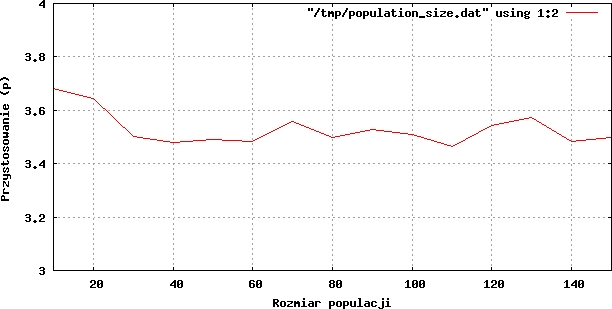
\includegraphics[width=.8\hsize]{fig/population_size}
\caption{Wpływ wielkości populacji na jakość rozwiązania}
\end{figure}

Wartości wag kryteriów zostały dobrane eksperymentalnie, tak aby wpływ poszczególnych kryteriów na końcowe rozwiązanie był jak najbardziej zrównoważony. Niektóre kryteria stanowią odchylenie od wartości optymalnej i ich wartości są stosunkowo niewielkie, w idealnym przypadku równe zeru. Inne natomiast to sumy częstotliwości, które przyjmują wartości o około 4 rzędy wielkości większe. Dlatego też wartości dla tych ostatnich zostały odpowiednio przeskalowane, poprzez dobranie dla nich wag o wartościach rzędu $10^{-4}$. Przyjęte zostały następujące wartości wag:
\newline
\begin{tabular}{ l l }
  \indent $ w_{finger} = 37,2 $ & \indent $ w_{row} = 33,3 $ \\
  \indent $ w_{hand\_alter} = 4,5 \cdot 10^{-4} $ & \indent $ w_{finger\_alter} = 1,6 \cdot 10^{-3} $ \\
  \indent $ w_{step} = 1,9 \cdot 10^{-4} $ & \indent $ w_{isf} = 2,5 \cdot 10^{-4} $ \\
  \indent $ w_{hand\_usage} = 71,4 $ & \\
\end{tabular}\newline

Zastosowanie strategii elitarnej przyspiesza zbieżność algorytmu, co obrazuje poniższy wykres. Rozmiar elity nie ma dużego wpływu na jakość rozwiązania końcowego, dopóki jest on niewielki. Dla rozmiaru elity większego niż kilka osobników, jakość rozwiązania pogarsza się.
\begin{figure}[!tbh]
\centering
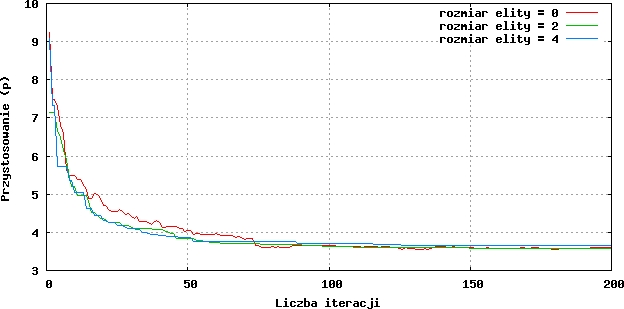
\includegraphics[width=.8\hsize]{fig/elite}
\caption{Wpływ zastosowania strategii elitarnej}
\end{figure}

Celem zastosowania operatora selekcji MMTS jest zrównoważenie wpływu poszczególnych składowych funkcji oceny, aby móc osiągnąć lepszy wynik dla wszystkich składowych w stosunku do innych rozwiązań, takich jak klawiatura Dvoraka. Dla standardowej selekcji turniejowej, po 100 uruchomieniach algorytmu przewaga w stosunku do klawiatury Dvoraka została osiągnięta średnio w 4,55 kryteriach na 7. Dla selekcji MMTS, współczynnik ten wyniósł 4,76 kryteriów na 7.

Zbadany został wpływ operatorów mutacji oraz krzyżowania na jakość najlepszego rozwiązania (wartość funkcji przystosowania $p$) znalezionego w wyniku uruchomienia algorytmu. Wyniki dla operatorów mutacji: zamiany (EM), zamiany z przemieszczeniem (DM), mutacji ze wstawianiem (ISM), prostej inwersji (SIM), inwersji (IVM) oraz z mieszaniem podlist (SM) przedstawiono w poniższej tabeli. Wyniki zostały uśrednione dla 10 uruchomień algorytmu.
\newline\newline
\begin{tabular}{ c | c }
  operator mutacji & najlepsza znaleziona wartość $p$ \\
  \hline
  EM  & 3,553 \\
  DM  & 3,73 \\
  SIM & 3,746 \\
  SM  & 3,876 \\
  IVM & 3,882 \\
  ISM & 4,301 \\
\end{tabular}\newline

Wyniki dla operatorów krzyżowania: cyklicznego (CX), z częściowym odwzorowaniem (PMX), bazującego na porządku (POS) oraz naprzemiennego (AP) przedstawiono poniżej, również uśrednione dla 10 uruchomień algorytmu.
\newline\newline
\begin{tabular}{ c | c }
  operator krzyżowania & najlepsza znaleziona wartość $p$ \\
  \hline
  PMX & 3,449 \\
  CX  & 3,509 \\
  POS & 3,543 \\
  AP  & 3,582 \\
\end{tabular}\newline

Największy wpływ na wyniki ma stosowanie operatora mutacji, natomiast krzyżowanie ma stosunkowo niewielkie znaczenie. Stosowanie samego operatora mutacji bez krzyżowania prowadzi do otrzymywania rozwiązań około 1\% gorszych w porównaniu do stosowania obu, natomiast samego krzyżowania bez mutacji, około 62\% gorszych.


%\pagebreak[2]

\section{Dane testowe}

Do obliczania oceny układów klawiatury dla języka polskiego został użyty zbiór tekstów powstały przez konkatenację 10 najpopularniejszych książek w języku polskim ze strony {\tt www.gutenberg.org}. Analogicznie, do oceny układów klawiatury dla języka angielskiego wykorzystano 10 najpopularniejszych książek w języku angielskim. Zbiór tekstów w języku polskim ma wielkość 1,9MB (kodowanie UTF-8), a w języku angielskim 5,4MB.

Cechy statystyczne tekstów uwzględniane w funkcji przystosowania, czyli częstotliwości występowania monografów oraz diagrafów, różnią się znacząco dla różnych języków. Na poniższym wykresie porównano częstotliwości występowania monografów w języku polskim oraz angielskim.

\begin{figure}[!tbh]
\centering
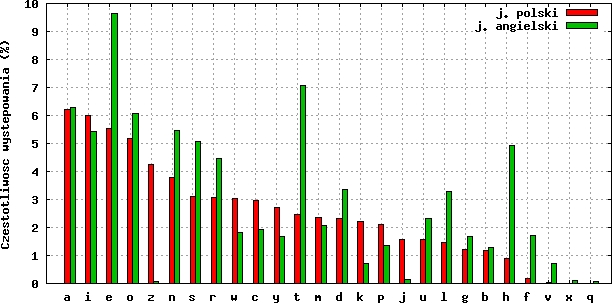
\includegraphics[width=.8\hsize]{fig/frequencies}
\caption{Porównanie częstotliwości występowania liter w języku polskim i angielskim}
\end{figure}

Pomimo pewnego podobieństwa, różnice są wyraźne, zwłaszcza w przypadku liter \emph{e}, \emph{z}, \emph{t} oraz \emph{h}. Jeszcze większe różnice widoczne są w przypadku diagrafów. Dla przykładu, najpopularniejsze pary znaków w języku angielskim, czyli \emph{he} oraz \emph{th}, w języku polskim nie występują prawie wcale. Analogicznie, często występujący w języku polskim dwuznak \emph{rz} jest niespotykany w języku angielskim. Warto zwrócić uwgę, że para \emph{th} jest bardzo łatwa do wpisania na klawiaturze Dvoraka. Porównanie częstotliwości występowania najczęstszych diagrafów w języku polskim i angielskim przedstawiono w tabeli poniżej.\newline

\begin{tabular}{ c | c | c }
  diagraf & język polski & język angielski \\
  \hline
  ie &	4,11\% &	0,30\% \\
  ni &	2,78\% &	0,26\% \\
  na &	1,64\% &	0,21\% \\
  rz &	1,61\% &	0,00\% \\
  cz &	1,58\% &	0,00\% \\
\end{tabular}
\begin{tabular}{ c | c | c }
  diagraf & język angielski & język polski \\
  \hline
  he &	3,73\% &	0,11\% \\
  th &	3,68\% &	0,00\% \\
  in &	2,39\% &	0,28\% \\
  er &	2,16\% &	0,68\% \\
  an &	2,10\% &	1,03\% \\
\end{tabular}\newline\newline

Ze względu na opisane wyżej różnice, wyniki algorytmu dla języka polskiego oraz angielskiego zostaną opisane osobno.


\section{Wyniki dla języka angielskiego}

Porównanie wartości funkcji przystosowania oraz jej składników dla różnych układów klawiatury przedstawiono w tabeli poniżej. Układ znaleziony przez algorytm genetyczny opisany w tej pracy oznaczono jako AG. SW to najlepsze rozwiązanie znalezione przez algorytm symulowanego wyżarzania \cite{Anderson:SimulatedAnnealing}, a AG2 - przez inny algorytm genetyczny opisany w artykule \cite{Call:2005:CME}.
\newline\newline
\begin{tabular}{ c | c | c | c | c | c | c }
  kryterium            & losowy & QWERTY & Dvorak & AG & SW   & AG2 \\
  \hline
  $p$			&  11,96 & 13,36 & 3,92 & 3,44 & 9,76 & 5,1 \\
  \hline
  $p_{finger} w_{finger}$                &   1,12 &  0,38 & 0,31 & 0,12 &  1,4 & 0,49 \\
  $p_{row} w_{row}$                      &    5,9 &  7,28 & 0,06 & 0,02 &  4,3 & 0,97 \\
  $p_{hand\_alter} w_{hand\_alter}$      &    1,1 &  1,11 & 0,81 & 0,79 & 0,78 & 0,81 \\
  $p_{finger\_alter} w_{finger\_alter}$  &   1,34 &  0,93 & 0,62 & 0,62 & 0,94 & 0,64 \\
  $p_{step} w_{step}$                    &   1,41 &  1,65 & 0,91 & 0,78 & 1,15 & 0,93 \\
  $p_{isf} w_{isf}$                      &   1,09 &  1,06 &  1,1 &  1,1 & 1,15 & 1,16 \\
  $p_{hand\_usage} w_{hand\_usage}$      & 0,0004 &  0,93 &  0,1 & 0,01 & 0,02 & 0,09 \\
\end{tabular}\newline\newline

\begin{figure}[!tbh]
\centering
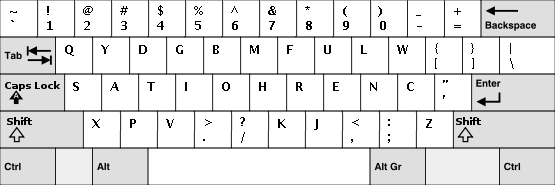
\includegraphics[width=.8\hsize]{fig/best_en}
\caption{Najlepszy układ klawiszy dla języka angielskiego znaleziony przez algorytm}
\end{figure}

\begin{figure}[!tbh]
\centering
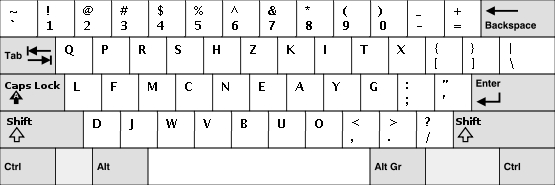
\includegraphics[width=.7\hsize]{fig/sw_en}
\end{figure}
\begin{figure}[!tbh]
\centering
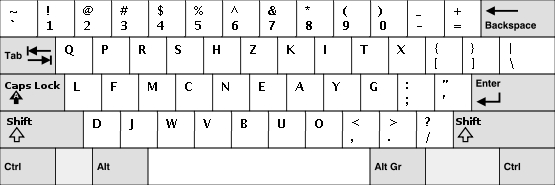
\includegraphics[width=.7\hsize]{fig/ag2_en}
\caption{Najlepsze rozwiązania algorytmów SW (na górze) oraz AG2 (na dole)}
\end{figure}

Ponieważ podczas projektowania układu QWERTY nie były uwzględniane kryteria ergonomiczne, należy spodziewać się że nie będzie on znacząco lepszy od losowo wygenerowanego układu klawiszy. Rzeczywiście, funkcja oceny nie różni się istotnie w tych przypadkach, a nawet jest gorsza dla QWERTY. Wyraźnie lepsze wyniki osiągnął układ Dvoraka, co nie jest zaskoczeniem biorąc pod uwagę fakt, że był on tworzony z myślą o języku angielskim, a kryteria stosowane przy jego projektowaniu w dużym stopniu pokrywają się z tymi użytymi w funkcji przystosowania. Najlepszy wynik znaleziony przez algorytm posiada ocenę o $12\%$ korzystniejszą od najlepiej ocenionego układu wśród pozostałych, jakim jest klawiatura Dvoraka. Algorytmy AG2 oraz SW uzyskały ocenę lepszą od QWERTY, ale też wyraźnie gorszą od Dvoraka. Jednym z powodów takiego stanu może być zastosowanie prostszych funkcji oceny w tych algorytmach - nie został w nich uwzględniony na przykład czynnik \emph{inboard stroke flow}. W przypadku algorytmu AG2 wpływ mógł mieć również dobór zbioru tekstów; największą jego część stanowiła Biblia Króla Jakuba, napisana językiem różniącym się znacznie od współczesnego angielskiego.

Większość układów klawiatury znalezionych przez algorytm przejawia wyraźną tendencję do umieszczania samogłosek po tej samej, lewej lub prawej stronie i na środkowym rzędzie. Pomysł Augusta Dvoraka, aby umieścić wszystkie samogłoski z lewej strony zaprojektowanego przez niego układu, znajduje tym samym niezależne potwierdzenie empiryczne (należy zwrócić uwagę, że algorytm nie posiada żadnej informacji o tym, które znaki są samogłoskami, a które spółgłoskami).

\begin{figure}[!tbh]
\centering
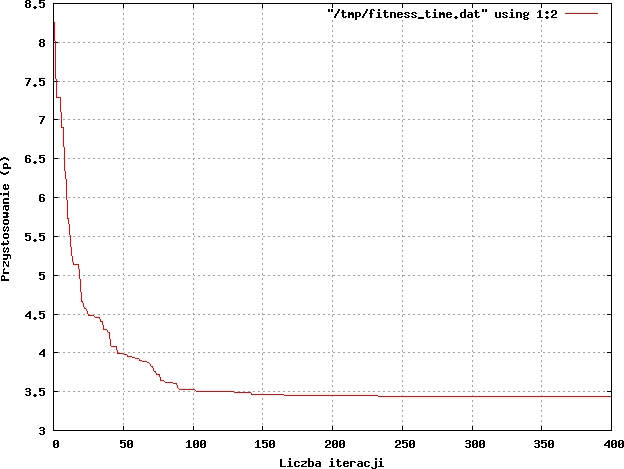
\includegraphics[width=.8\hsize]{fig/fitness_time_en}
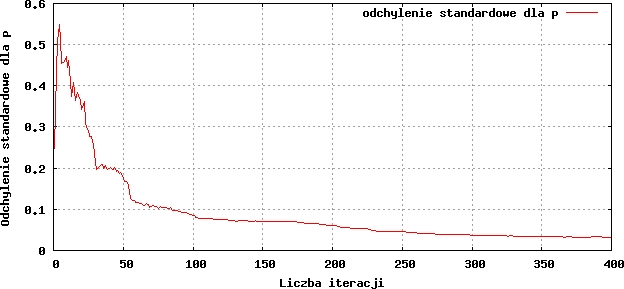
\includegraphics[width=.8\hsize]{fig/std_dev_time_en}
\caption{Ewolucja maksymalnego przystosowania w populacji oraz jego odchylenia standardowego. Wyniki uśredniono dla 30 wykonań algorytmu.}
\end{figure}

Różnice między poszczególnymi układami są szczególnie widoczne w przypadku wykorzystania rzędów klawiszy. Szczegółowe różnice przedstawiono w poniższej tabeli:\newline\newline
\begin{tabular}{ c | c | c | c | c | c | c }
  rząd klawiszy   & losowy & QWERTY & Dvorak & AG &     SW   & AG2 \\
  \hline
  górny           & 40,5\% & 49,1\% & 22,9\% & 22,0\% & 35,9\% & 18,6\% \\
  środkowy        & 36,5\% & 33,5\% & 68,3\% & 70,9\% & 41,7\% & 62,1\% \\
  dolny           &   23\% & 17,4\% &  8,8\% &  7,1\% & 22,4\% & 19,3\% \\
\end{tabular}\newline

W przypadku układu QWERTY zdecydowanie zbyt duży nacisk położony jest na górny rząd klawiszy, podczas gdy najkorzystniejszy środkowy rząd jest wykorzystany w zaledwie jednej trzeciej. Jest to jedna z największych wad tego układu; nietrudno jest wygenerować losowo układ z lepszym rozkładem. Dobrze widoczne są zalety klawiatury Dvoraka, która posiada rozkład zbliżony do optymalnego, wykorzystując w bardzo dużym stopniu rząd środkowy. Mimo to, układ klawiatury znaleziony przez algorytm poprawił ten wynik jeszcze bardziej.

Poniższa tabela przedstawia różnice w stopniu użycia poszczególnych palców pomiędzy testowanymi układami klawiszy:\newline\newline
\begin{tabular}{ c | c | c | c | c | c | c | c | c }
                & lewy & lewy  & lewy & lewy & prawy & prawy & prawy & prawy \\
  układ         & mały & serd. & śr. & wsk. & wsk. & śr. & serd. & mały \\
  \hline
  losowy        & 14\% & 2\% & 10\% & 21\% & 16\% & 24\% & 9\%  & 4\% \\
  QWERTY        &  8\% & 9\% & 18\% & 21\% & 20\% & 9\%  & 13\% & 2\% \\
  Dvorak        &  8\% & 9\% & 13\% & 14\% & 18\% & 13\% & 13\% & 10\% \\
  AG            &  6\% & 9\% & 15\% & 19\% & 18\% & 15\% & 10\% & 8\% \\
  SW            &  8\% & 4\% & 10\% & 24\% & 31\% & 10\% & 12\% & 0\% \\
  AG2           &  8\% & 9\% & 12\% & 22\% & 23\% & 11\% &  9\% & 8\% \\
\end{tabular}\newline

Tym razem układ QWERTY sprawdza się lepiej od losowo wygenerowanego. Rozkłady dla klawiatury Dvoraka oraz układu znalezionego przez algorytm są jednak bardziej równomierne.


\section{Wyniki dla języka polskiego}

Porównanie wartości funkcji przystosowania oraz jej składników dla różnych układów klawiatury:\newline\newline
\begin{tabular}{ c | c | c | c | c }
  kryterium         & losowy & QWERTY & Dvorak & AG \\
  \hline
  $p$			& 7,25 & 8,44 & 3,64 & 1,06 \\
  \hline
  $p_{finger} w_{finger}$                & 0,72 & 0,77 & 0,94 & 0,05 \\
  $p_{row} w_{row}$                      & 4,66 & 5,64 & 1,07 & 0,03 \\
  $p_{hand\_alter} w_{hand\_alter}$      & 0,35 & 0,37 & 0,28 & 0,23 \\
  $p_{finger\_alter} w_{finger\_alter}$  & 0,35 & 0,31 & 0,22 & 0,14 \\
  $p_{step} w_{step}$                    & 0,52 & 0,62 & 0,46 & 0,23 \\
  $p_{isf} w_{isf}$                      & 0,36 & 0,36 & 0,38 & 0,37 \\
  $p_{hand\_usage} w_{hand\_usage}$      & 0,30 & 0,37 & 0,28 & 0,002 \\
\end{tabular}\newline\newline

\begin{figure}[!tbh]
\centering
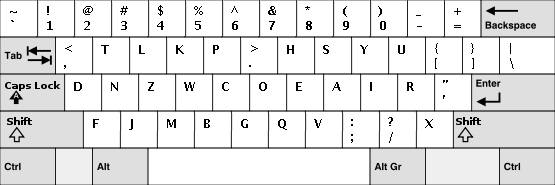
\includegraphics[width=.8\hsize]{fig/best_pl}
\caption{Najlepszy układ klawiszy dla języka polskiego znaleziony przez algorytm}
\end{figure}

Układ klawiatury Dvoraka był zaprojektowany z myślą o języku angielskim, dlatego należy się spodziewać że wynik dla języka polskiego nie będzie optymalny. Rzeczywiście, układ Dvoraka jest nadal lepszy od losowo wygenerowanego lub QWERTY, ale bardzo daleki od optimum. Układ klawiszy wygenerowany przez algorytm jest natomiast wyraźnie lepszy od wszystkich pozostałych, co daje znaczącą przewagę w porównaniu z wynikami dla języka angielskiego.

Różnice między poszczególnymi układami ze względu na wykorzystanie rzędów klawiszy przedstawiono w poniższej tabeli:\newline\newline
\begin{tabular}{ c | c | c | c | c}
  rząd klawiszy   & losowy & QWERTY & Dvorak & AG \\
  \hline
  górny           & 33,8\% & 44,7\% & 25,0\% & 29,0\% \\
  środkowy        & 35,5\% & 30,3\% & 54,0\% & 61,9\% \\
  dolny           & 30,7\% & 25,0\% & 21,0\% &  9,1\% \\
\end{tabular}\newline

W przypadku układu QWERTY, sytuacja wygląda jeszcze gorzej niż dla języka angielskiego: udział bardzo niekorzystnego rzędu dolnego wzrósł, a rzędu środkowego spadł do mniej niż jednej trzeciej. Wynik klawiatury Dvoraka również się pogorszył, co nie jest zaskakujące, ale nadal jest lepszy od losowo wygenerowanego rozwiązania. Przewaga rozwiązania znalezionego przez algorytm, niewielka w przypadku języka angielskiego, tym razem jest bardziej wyraźna.

Poniższa tabela przedstawia różnice w stopniu użycia poszczególnych palców pomiędzy testowanymi układami klawiszy:\newline\newline
\begin{tabular}{ c | c | c | c | c | c | c | c | c}
                & lewy & lewy      & lewy     & lewy       & prawy      & prawy    & prawy     & prawy \\
  układ         & mały & serd. & śr. & wsk. & wsk. & śr. & serd. & mały \\
  \hline
  losowy        &  10\% & 6\% & 8\% & 20\% &   19\% & 13\% & 17\% & 9\% \\
  QWERTY        &  16\% & 9\% & 16\% & 11\% &  17\% & 13\% & 14\% & 3\% \\
  Dvorak        &  10\% & 10\% & 12\% & 20\% & 11\% & 12\% & 9\% & 16\% \\
  AG            &  5\% & 11\% & 14\% & 18\% &  19\% & 15\% & 12\% & 6\% \\
\end{tabular}\newline\newline

Ze względu na różnice w częstotliwości występowania liter, wyniki dla układów QWERTY oraz Dvorak są znacznie gorsze niż w przypadku języka angielskiego. QWERTY kładzie zbyt duży nacisk na lewy mały palec, który służy do wpisywania popularnych w języku polskim liter \emph{a} oraz \emph{z}. Z kolei klawiatura Dvoraka przeciąża prawy mały palec, obsługujący litery \emph{l}, \emph{s} oraz \emph{z}, w zbyt małym stopniu natomiast wykorzystując prawy palec wskazujący. Problemy te nie dotyczą układu wygenerowanego przez algorytm.

\begin{figure}[!tbh]
\centering
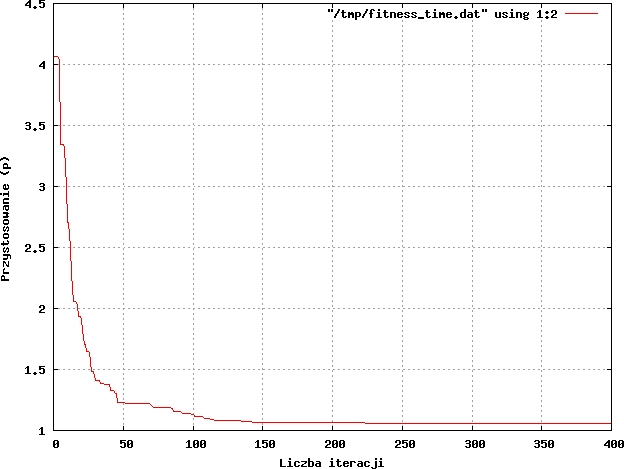
\includegraphics[width=.8\hsize]{fig/fitness_time_pl}
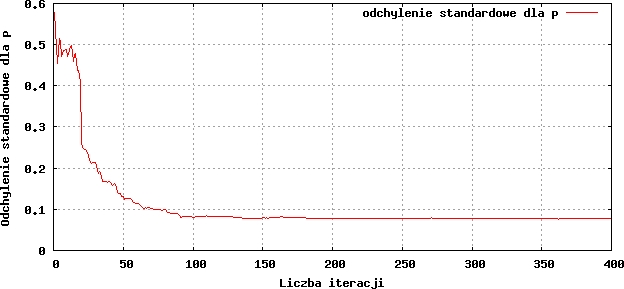
\includegraphics[width=.8\hsize]{fig/std_dev_time_pl}
\caption{Ewolucja maksymalnego przystosowania w populacji oraz jego odchylenia standardowego. Wyniki uśredniono dla 30 wykonań algorytmu.}
\end{figure}


% zakończenie
\summary

\section{Konkluzje}

Projektowanie optymalnego układu klawiatury (KAP - Keyboard Arrangement Problem) jest złożonym problemem, który wymaga uwzględnienia wielu czynników wpływających na ergonomię pisania. Rozwiązywanie go bez pomocy komputera jest zajęciem bardzo czasochłonnym i nie gwarantuje znalezienia optymalnego rozwiązania. Co więcej, dla każdego języka naturalnego problem musi być podejmowany od nowa, ze względu na różnice w częstotliwości występowania liter oraz ich par pomiędzy językami. Jak pokazują wyniki, dobór tekstów do których pisania ma być przystosowany dany układ klawiszy ma bardzo duży wpływ na jego ocenę.

Ogromna ilość potencjalnych rozwiązań oraz trudność w optymalizowaniu wielu czynników jednocześnie sprawiają, że KAP jest dobrym kandydatem na zastosowanie algorytmu genetycznego. Naturalnym sposobem reprezentacji chromosomu jest permutacja, co pozwala na stosowanie operatorów genetycznych wypróbowanych na innych zagadnieniach optymalizacji kombinatorycznej, takich jak problem komiwojażera.

Uzyskane wyniki pokazują jasno, że istnieją układy klawiszy lepsze od tych pozostających w powszechnym użyciu i algorytmy genetyczne potrafią znajdywać je stosunkowo szybko. Najlepszym spośród powstałych dotychczas układów okazał się układ Dvoraka. Dla języka angielskiego, najlepszy układ znaleziony przez algorytm uzyskał korzystniejszą ocenę w stosunku do klawiatury Dvoraka pod względem wszystkich czynników branych pod uwagę w funkcji oceny. W przypadku wyników dla języka polskiego, różnice są jeszcze bardziej widoczne. Pewnym zaskoczeniem są słabe wyniki osiągnięte przez inne algorytmy (SW, AG2), szczególnie w porównaniu do klawiatury Dvoraka. Może to wynikać z zastosowania prostszych kryteriów oceny rozwiązań oraz mało różnorodnych zbiorów tekstów przez ich autorów.

Istnieje niewiele badań empirycznych na temat czynników wpływających na ergonomię pisania, a te istniejące najczęściej przeprowadzane były na niewielką skalę. Dlatego też kryteria przyjęte podczas oceny rozwiązań przedstawionego algorytmu z pewnością nie stanowią ostaniego słowa w tej dziedzinie. Stanowią one jednak pewien punkt wyjścia i można je w łatwy sposób zmodyfikować w miarę pojawiania się kolejnych danych w dziedzinie ergonomii.

\section{Plany dalszych badań}

Użyty algorytm był stworzony z myślą o technice pisania bezwzrokowego. Interesującym problemem byłoby przystosowanie go do techniki pisania jednym palcem, która znajduje zastosowanie między innymi podczas pisania na urządzeniach posiadających ekran dotykowy. W tym celu można by zmodyfikować funkcję oceny w taki sposób, żeby algorytm minimalizował długość ścieżki jaką musi przebyć palec (lub rysik albo podobne urządzenie) podczas przepisywania zadanego tekstu. Tego typu zadanie można sprowadzić do zagadnienia Quadratic Assignment Problem (QAP), będącego jednym z klasycznych problemów optymalizacji kombinatorycznej~\cite{Ji_asolution}. Algorytmy genetyczne były już wykorzystywane z pewnymi sukcesami do rozwiązywania QAP~\cite{Misevicius200465}.

Podczas projektowania funkcji oceny ograniczono się do kryteriów ergonomicznych mających na celu ułatwienie pisania zwykłego tekstu. Możliwe byłoby wprowadzenie dodatkowych kryteriów mających znaczenie dla klawiatury komputerowej. Na przykład, układ klawiatury Colemak został stworzony z myślą o łatwym dostępie do standardowych skrótów klawiszowych stosowanych w oprogramowaniu, takich jak Ctrl-C, Ctrl-X i Ctrl-V.

Warto byłoby również zbadać wpływ rodzaju zbioru tekstów na wynikowe układy klawiatury. W tym przypadku wykorzystano teksty literackie w dwóch językach. Innym przykładem byłoby zastosowanie kodu źródłowego w różnych językach programowania, w celu stworzenia układu klawiatury przystosowanego specjalnie dla programisty.

Algorytm genetyczny jaki został użyty z pewnością mógłby zostać rozwinięty i ulepszony. Korzystne byłoby przetestowanie większej ilości operatorów genetycznych oraz zaawansowanych technik, takich jak niszowość lub zmienność rozmiaru populacji w czasie. W szczególności, warto byłoby porównać otrzymane wyniki z wynikami uzyskanymi przez zastosowanie specjalistycznych wariantów algorytmów genetycznych zaprojektowanych z myślą o optymalizacji wielokryterialnej, takich jak NSGA, NSGA-II lub VEGA.


% załączniki (opcjonalnie):
\appendix
\chapter{Część programowa}

Do pracy dołączono program w języku Java, stanowiący implementację opisanego w niej algorytmu.

Sposób uruchomienia programu:\newline
\texttt{java -cp build/classes mdettla.keyboard.ga.GAKeyboard [parametry] PLIK...}

Jako argument \texttt{PLIK...} należy podać ścieżki do plików tekstowych, na podstawie których zostaną obliczone statystyki używane w funkcji oceny. Teksty dla języka angielskiego znajdują się w katalogu \emph{src/mdettla/keyboard/ga/resources/en}, a dla języka polskiego w katalogu \emph{src/mdettla/keyboard/ga/resources/pl}.

Dostępne są następujące parametry pozwalające wpływać na działanie algorytmu:
\begin{itemize}
  \item \texttt{populationSize} - rozmiar populacji
  \item \texttt{generationsCount} - ilość iteracji
  \item \texttt{eliteSize} - rozmiar elity
  \item \texttt{tournamentSize} - rozmiar turnieju
  \item \texttt{mutationProbability} - prawdopodobieństwo zajścia mutacji
  \item \texttt{mutationOperator} - operator mutacji (należy podać nazwę jednej z klas znajdujących się w katalogu \emph{src/mdettla/jga/operators/mutation})
  \item \texttt{crossoverProbability} - prawdopodobieństwo zajścia krzyżowania
  \item \texttt{crossoverOperator} - operator krzyżowania (należy podać nazwę jednej z klas znajdujących się w katalogu \emph{src/mdettla/jga/operators/crossover})
  \item \texttt{selectionFunction} - funkcja selekcji (należy podać nazwę jednej z klas znajdujących się w katalogu \emph{src/mdettla/jga/operators/selection})
\end{itemize}

Przykład uruchomienia programu:\newline
\texttt{java -cp build/classes mdettla.keyboard.ga.GAKeyboard \textbackslash \newline
\indent populationSize=100 mutationProbability=0.5 \textbackslash \newline
\indent mutationOperator=mdettla.jga.operators.mutation.SwapMutation \textbackslash \newline
\indent src/mdettla/keyboard/ga/resources/pl/*}


% literatura (obowiązkowo):
\bibliographystyle{unsrt}
\bibliography{bib}

% spis tabel (jeżeli jest potrzebny):
%\listoftables

% spis rysunków (jeżeli jest potrzebny):
\listoffigures

\oswiadczenie

\end{document}
